\section{Messergebnisse und Auswertung}

\subsection{Zählrohrcharakteristik mit \uran}
\label{sub:eval:uran}
Die gemessene Abhängigkeit der Zählrate $n$ von \uran\, ohne Untergrund von der Zählrohrspannung $U$ wird in der Abbildung \ref{img:char:uran} gezeigt.
Von der gemessenen Zählrate $\hat{n}$ muss der Untergrund $u$ abgezogen werden, um die echte Zählrate $n$ zu erhalten: $n = \hat{n}- u$. Der 
Fehler auf die echte Zählraten $n$ beträgt nach \autoref{eq:counts:errors}
\begin{equation}
  s_n=\sqrt{s_{\hat{n}}{}^2+s_u{}^2}=\sqrt{\frac{\hat{n}}{t_{\hat{n}}}+\frac{u}{t_u}}
\end{equation}
wobei $t_{\hat{n}}$ und $t_u$ der Messzeit pro Messpunkt der gemessenen Zählrate bzw. des Untergrunds entspricht. \\
Jedoch sind die Fehler der Zählrate des Urans wegen der logarithmischen Skala nicht mehr gut zu erkennen, weshalb sie in der Abbildung nicht 
eingezeichnet wurden.
\begin{figure}[H]
\begin{center}
  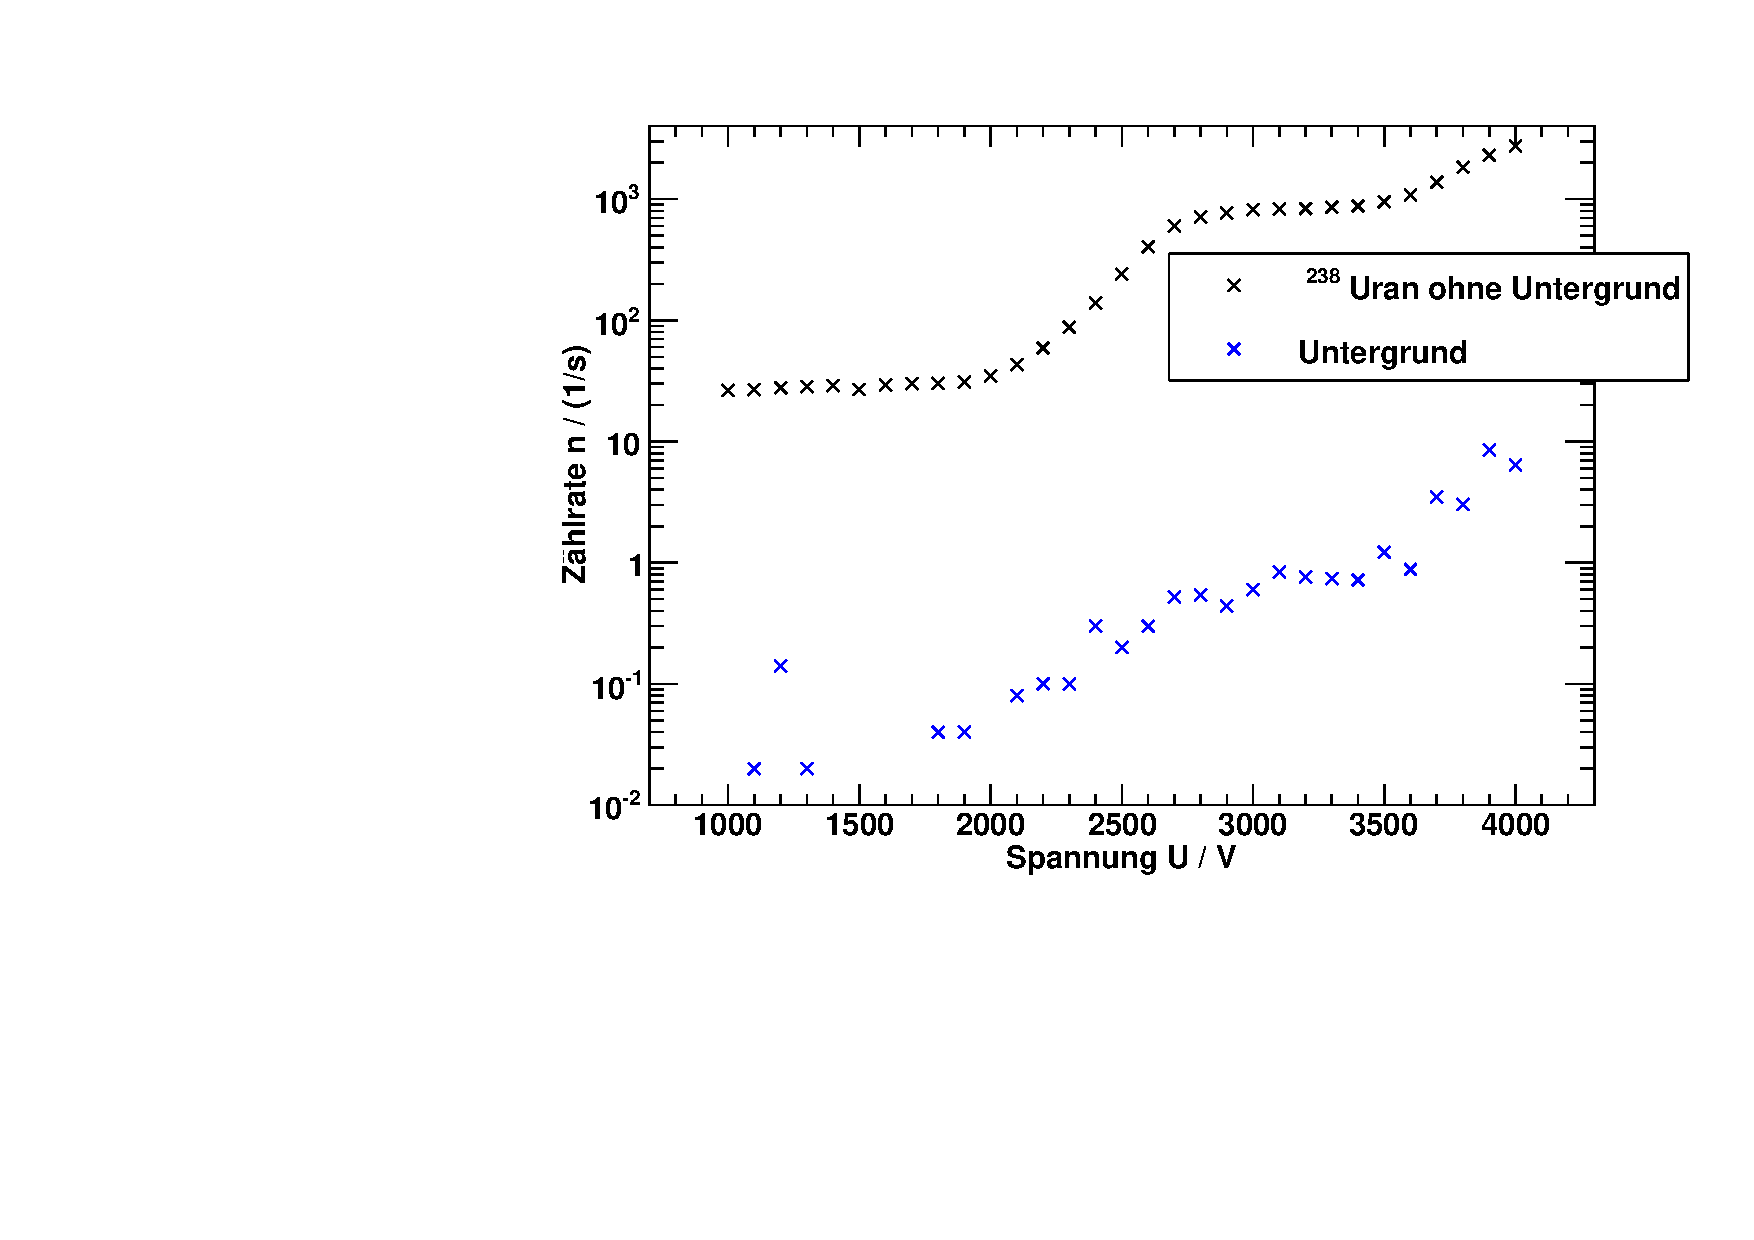
\includegraphics[width=15cm]{../img/Uran238_Charakteristik.pdf}
  \caption[Zählrohrcharakteristik mit \uran]{Zählrohrcharakteristik mit \uran\, und Untergrund}
  \label{img:char:uran}
\end{center}
\end{figure}
Man erkennt gut das $\alpha$-Plateau bis ca. $2000\,V$ und das $\beta$-Plateau von $2800\,V$ bis $3500\,V$, welche durch die 
unterschiedlichen Energien der beiden Strahlungen verursacht werden. Des weiteren wurde die Zählrate des Untergrundes in der gleiche Abbildung 
\ref{img:char:uran} abgebildet. Der Anstieg der Zählrate des Untergrundes, verursacht von der Zählrohrspannung, lässt sich gut erkennen. Allerdings 
sieht man auch die statistischen Schwankungen in der Zählrate des Untergrundes (die Messpunkte mit $n = 0 $ lassen sich auf der logarithmischen 
Skala nicht darstellen), da die einzelnen Messpunkte nur in einer geringen Zeitspanne ($t=50\,$s) aufgenommen wurden. Für eine glattere Kurve wäre 
eine längere Messzeit erforderlich gewesen.
\subsection{Bestimmung der Halbwertszeit von \samarium}
Alle Zählraten in diesem Abschnitt sind schon die echten Zählraten, also die gemessenen Zählraten vom Untergrund bereinigt. 
Die Werte und ihre Fehler wurden wie in \ref{sub:eval:uran} beschrieben berechnet.
\ref{sub:eval:uran} beschrieben bestimmt.
\subsubsection{$\alpha$-Plateau von \samarium}
\begin{figure}[H]
\begin{center}
  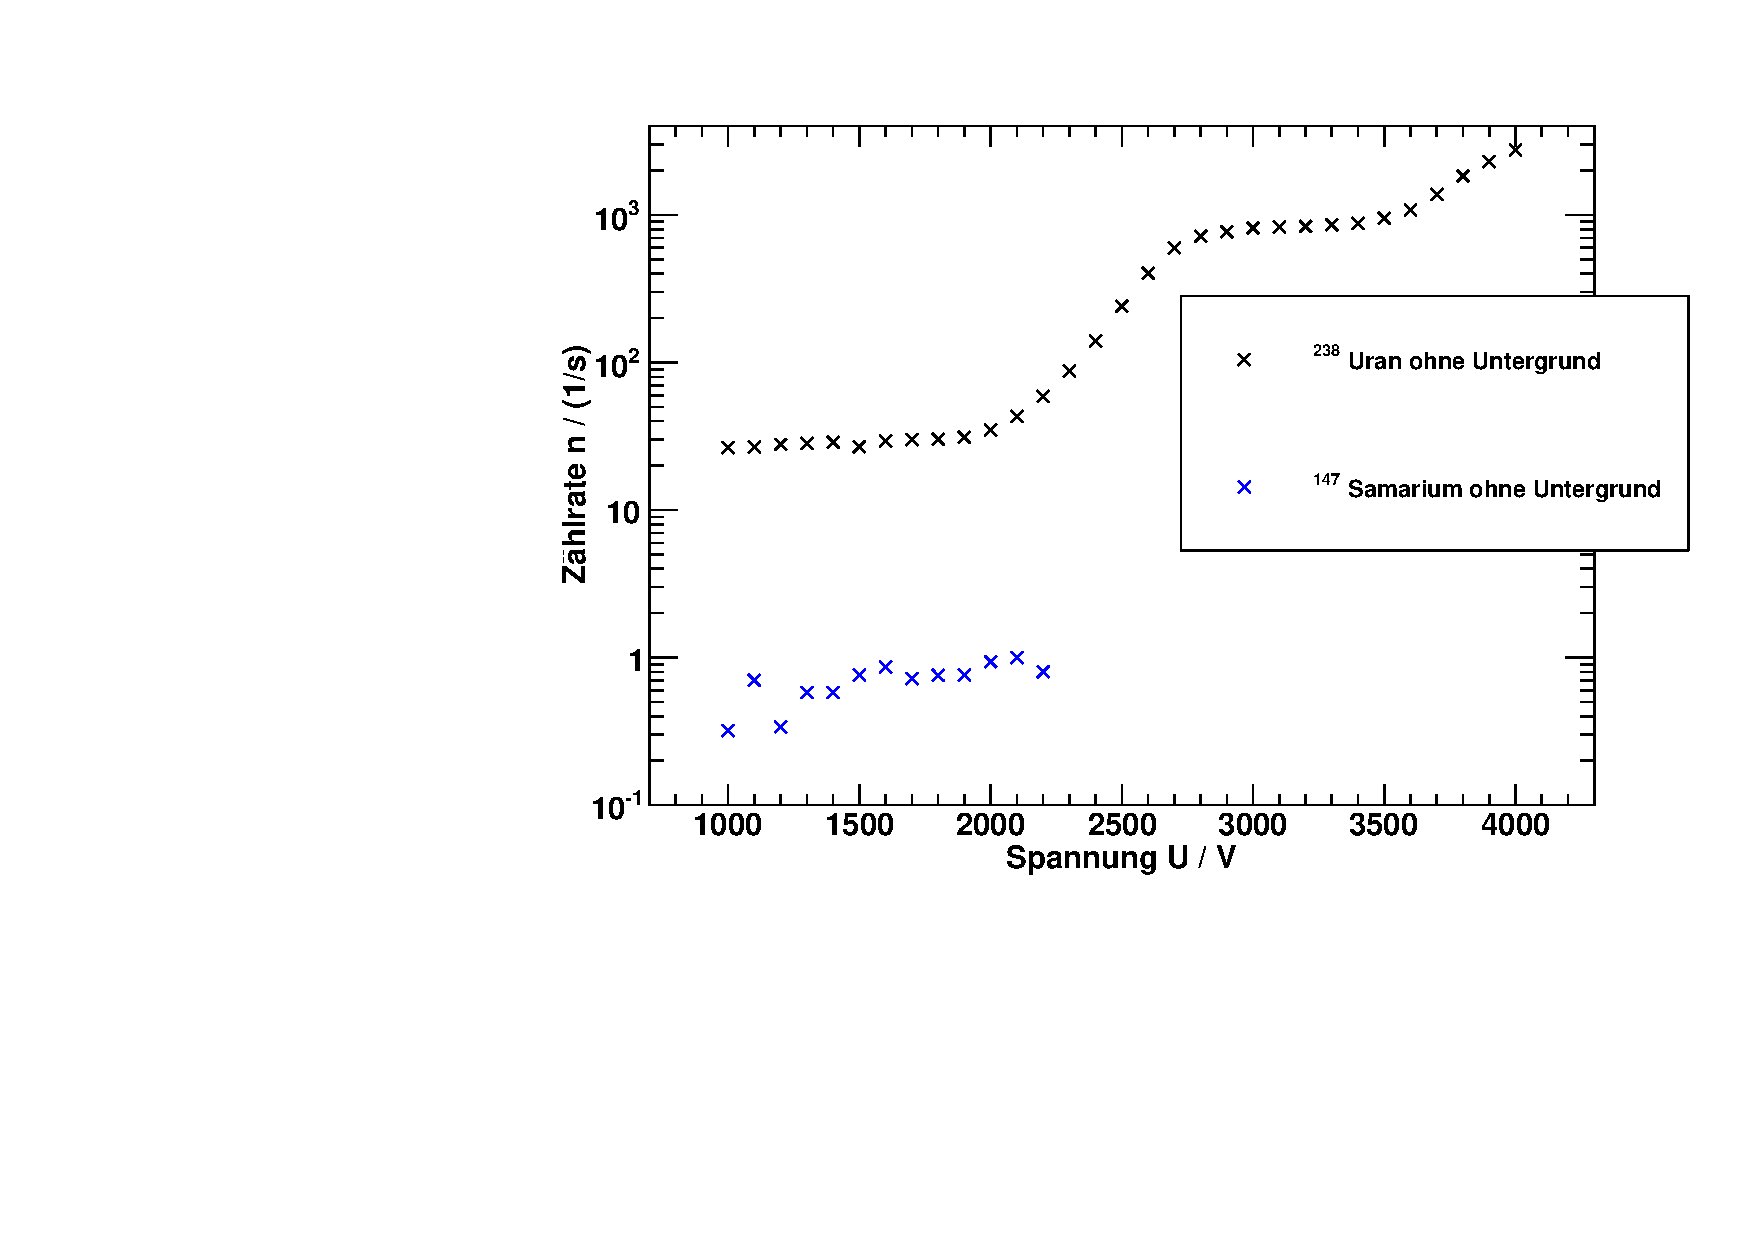
\includegraphics[width=15cm]{../img/Samarium147_Charakteristik.pdf}
  \caption[$\alpha$-Plateau mit \samarium]{$\alpha$-Plateau von \samarium} %TODO bessere beschreibung
  \label{img:char:samarium}
\end{center}
\end{figure}
In \autoref{img:char:samarium} ist das $\alpha$-Plateau von \samarium\, im Vergleich zur Zählrohrcharakteristik von \uran\, dargestellt worden. 
Man erkennt trotz einiger Schwankungen den Plateaucharakter des aufgenommenen Ausschnitts. Möchte man die Schwankungen verringern, so ist eine 
längere Dauer der Messzeit erforderlich.

\subsubsection{Messung der Flächen}
Die Durchmesser $d$ der verschiedenen Flächen wurden je $N = 6$ mal mit einer Schiebelehre (Fehler $s_d = 0.005$ cm) gemessen. Der Mittelwert $\bar{d}$ berechnet sich mit
\begin{equation}
  \bar{d} = \frac{1}{n} \sum_{i=1}^{n} d_i
\end{equation}
Nun gibt es zwei Arten von Fehlern für den mittleren Durchmesser, der eine entspricht der Standardabweichung\footnote{Allerdings muss hier mit 
dem Gewichtungsfaktor $\frac{1}{N-1}$ gerechnet werden, da aus dem gleichen Datensatz schon der Mittelwert berechnet wurde und somit ein Freiheitsgrad 
weniger verfügbar ist.} 
und der andere lässt sich aus dem Fehler der Einzelmessung berechnen.
\begin{equation}
  s_{\bar{d}, \text{stat}} = \sqrt{\frac{1}{N-1} \sum_{n=1}^{N} \left( d_i - \bar{d} \right)^2} \qquad \text{und} \qquad 
  s_{\bar{d}} = \frac{s_d}{\sqrt{N}} 
\end{equation}
%TODO wieso nicht beide Fehler quatratisch addieren?
Wie man in \autoref{tab:data:samarium:diameter} sehen kann, ist der statistische Fehler immer größer oder gleicht dem Fehler, der durch die Einzelmessungen 
verursacht wird. Deshalb haben wir im Folgenden mit dem statistischen Fehler die Fehler der abhängigen Größen berechnet.
\begin{table}[H]
\caption{Mittlere Durchmesser $\bar{d}$ mit verschiedenen Fehlern}
\begin{center}
\begin{tabular}{|c|c|c|}
  \hline
  \rule{0pt}{1em} Durchmesser $\bar{d}$ / cm & $s_{\bar{d}, \text{stat}} / \text{cm}$ & $s_{\bar{d}} / \text{cm}$  \\ \hline % strech height with \rule so that bar is visible
  0.9983 & 0.0068 & 0.002 \\ \hline
  1.6992 & 0.0058 & 0.002 \\ \hline
  2.8792 & 0.0020 & 0.002 \\ \hline
\end{tabular}
\end{center}
\label{tab:data:samarium:diameter}
\end{table}
Im Folgenden wird der mittlere Durchmesser mit $d$ und der Fehler mit $s_d$ bezeichnet.
\subsubsection{Bestimmung der Halbwertszeit von \samarium ~aus den einzelnen Flächen}
\label{subsub:samarium:halflife:single}
Die Fläche und ihr Fehler berechnen sich nun mit
\begin{equation}
  F = \pi  \cdot \left( \frac{d}{2} \right)^2 , \qquad 
  s_F = F \cdot \sqrt{ \left( \frac{\partial F}{\partial d} \cdot s_d \right)^2 } = \frac{d}{2} \cdot \pi \cdot s_d
\end{equation}
In \autoref{tab:data:samarium:area} sind die verschiedenen Flächen mit zugehörigen Fehlern aufgelistet.
\begin{table}[H]
\caption{Verschiedene Fl"achen f"ur die Samariummessung}
\begin{center}
\begin{tabular}{|c|c|c|c|}
  \hline
  Durchmesser $d$ / cm & $s_d$ / cm & Fl"ache $F / \text{cm}^2$ & $s_F / \text{cm}^2$ \\ \hline 
  0.9983 & 0.0068 & 0.7828 & 0.0107 \\ \hline
  1.6992 & 0.0058 & 2.2676 & 0.0156 \\ \hline
  2.8792 & 0.0020 & 6.5106 & 0.0092 \\ \hline
\end{tabular}
\end{center}
\label{tab:data:samarium:area}
\end{table}

Die Zählrate $n$ hängt nach \autoref{eq:nAFR4} von der Fläche $F$ folgendermaßen ab:
\begin{equation}
\label{eq:samarium:counts_eval}
  n(F) = \frac{A_V \cdot F \cdot R}{4} \Rightarrow A_V = \frac{4 \cdot n}{F \cdot R}
\end{equation}
Daraus lässt sich die Halbwertszeit mit \autoref{eq:samarium:halflife} bestimmen:
\begin{equation}
  \label{eq:samarium:halflife_eval}
  T_{1/2}({}^{147}Sm) = \frac{\ln 2}{2} \cdot
      \frac{\rho_{\text{Sm}_2\text{O}_3} \cdot R_{\text{Sm}_2\text{O}_3} \cdot N_A \cdot h_{\text{rel}}}{M_{\text{Sm}_2\text{O}_3}} 
  	  \cdot \frac{F}{n} = const. \cdot \frac{F}{n}
\end{equation}
mit $N_A$ Avogadrokonstante, $h_{\text{rel}} = 0.1487$ natürlicher Häufigkeit von Samarium und $M_{\text{Sm}_2\text{O}_3} = 348.717$ u der 
Molaren Masse von $\text{Sm}_2\text{O}_3$.
Der Faktor $\rho_{\text{Sm}_2\text{O}_3} \cdot R_{\text{Sm}_2\text{O}_3}$ ist eine Konstante und wurde in \autoref{eq:samarium:Rrho} berechnet:
\begin{equation}
  R \cdot \rho = 4.025 \cdot 10^{-3} \, \text{g/cm}^2
\end{equation}
In \autoref{tab:data:samarium} sind die Messdaten der Zählraten für die verschiedenen Flächen aufgelistet.
\begin{table}[H]
\caption{Z"ahlraten von \samarium~f"ur verschiedene Fl"achen mit Fehlern}
\begin{center}
\begin{tabular}{|c|c|c|c|}
  \hline
  Fl"ache $F / \text{cm}^2$ & $s_F / \text{cm}^2$ & Z"ahlrate $n / (1/\text{s})$ & $s_n / (1/\text{s})$ \\ \hline 
  0.7828 & 0.0107 & 0.139 & 0.010 \\ \hline
  2.2676 & 0.0156 & 0.290 & 0.014 \\ \hline
  6.5106 & 0.0092 & 0.678 & 0.026 \\ \hline
\end{tabular}
\end{center}
\label{tab:data:samarium}
\end{table}

Daraus lassen sich folgende Halbwertszeiten berechnen:
\begin{gather}
  T_{1/2}(F=0.783 \text{ cm}^2) = (0.639 \pm 0.05)\cdot 10^{11} \text{ a} \\
  T_{1/2}(F=2.268 \text{ cm}^2) = (0.888 \pm 0.04)\cdot 10^{11} \text{ a}\\
  T_{1/2}(F=6.5106 \text{ cm}^2) = (1.09 \pm 0.04)\cdot 10^{11} \text{ a}
\end{gather}
Man erkennt, dass die Werte für die Halbwertszeiten mit der Fläche zunehmen, was nicht dem theoretischen Modell entspricht (die Abhängigkeit der 
Fläche wurde schon in der Formel berücksichtigt und es werden deshalb ungefähr gleiche Werte erwartet). Außerdem ist der Unterschied der ersten und letzten 
Halbwertszeit $59\%$. Deshalb wird im nächsten Abschnitt versucht, die Halbwertszeit mit einer anderen Methode zu bestimmen, 
um etwaige systematische Fehler herauszufiltern.

\subsubsection{Bestimmung der Halbwertszeit von \samarium ~mit einer Ausgleichsgeraden}
Eine Ausgleichsgerade lässt sich mit nur drei Messpunkten nicht so exakt bestimmen, jedoch wurde wegen der großen Unstimmigkeit der Fehler 
zueinander eine andere Methode zur Bestimmung der Halbwertszeit gesucht.
Aus \autoref{eq:samarium:halflife_eval} folgt
\begin{equation}
   n = \frac{\ln 2}{2} \frac{R \cdot \rho \cdot N_A \cdot h_{\text{rel}}}{M_{\text{Sm}_2\text{O}_3} \cdot T_{1/2}({}^{147}\text{Sm})} \cdot F
\end{equation}
Es wird ein Polynom ersten Grades angesetzt:
\begin{equation}
  n(F) = a + b \cdot F
\end{equation}
wobei man mit der Steigung $b$ die Halbwertszeit berechnen kann
\begin{equation}
  T_{1/2}({}^{147}\text{Sm}) = \frac{\ln 2}{2} \frac{R \cdot \rho \cdot N_A \cdot h_{\text{rel}}}{M_{\text{Sm}_2\text{O}_3} \cdot b}
\end{equation}
Der Fehler folgt aus dem Fehler der Steigung $s_b$
\begin{equation}
  s_{T_{1/2}} = T_{1/2}({}^{147}\text{Sm}) \cdot \frac{s_b}{b}
\end{equation}
Der Achsenabschnitt $a$ ist im theoretischen Modell nicht erhalten und sollte daher im Idealfall verschwinden. \\[\baselineskip]
Die Kurvenanpassung liefert
\begin{gather}
  a = (0.068  \pm 0.012 ) \cdot \frac{1}{\text{s}} \\
  b = (0.0947 \pm 0.0048) \cdot \frac{1}{\text{s}\cdot \text{cm}^2}
\end{gather}
und ist in \autoref{img:samarium:areafit} graphisch dargestellt. 
\begin{figure}[H]
\begin{center}
  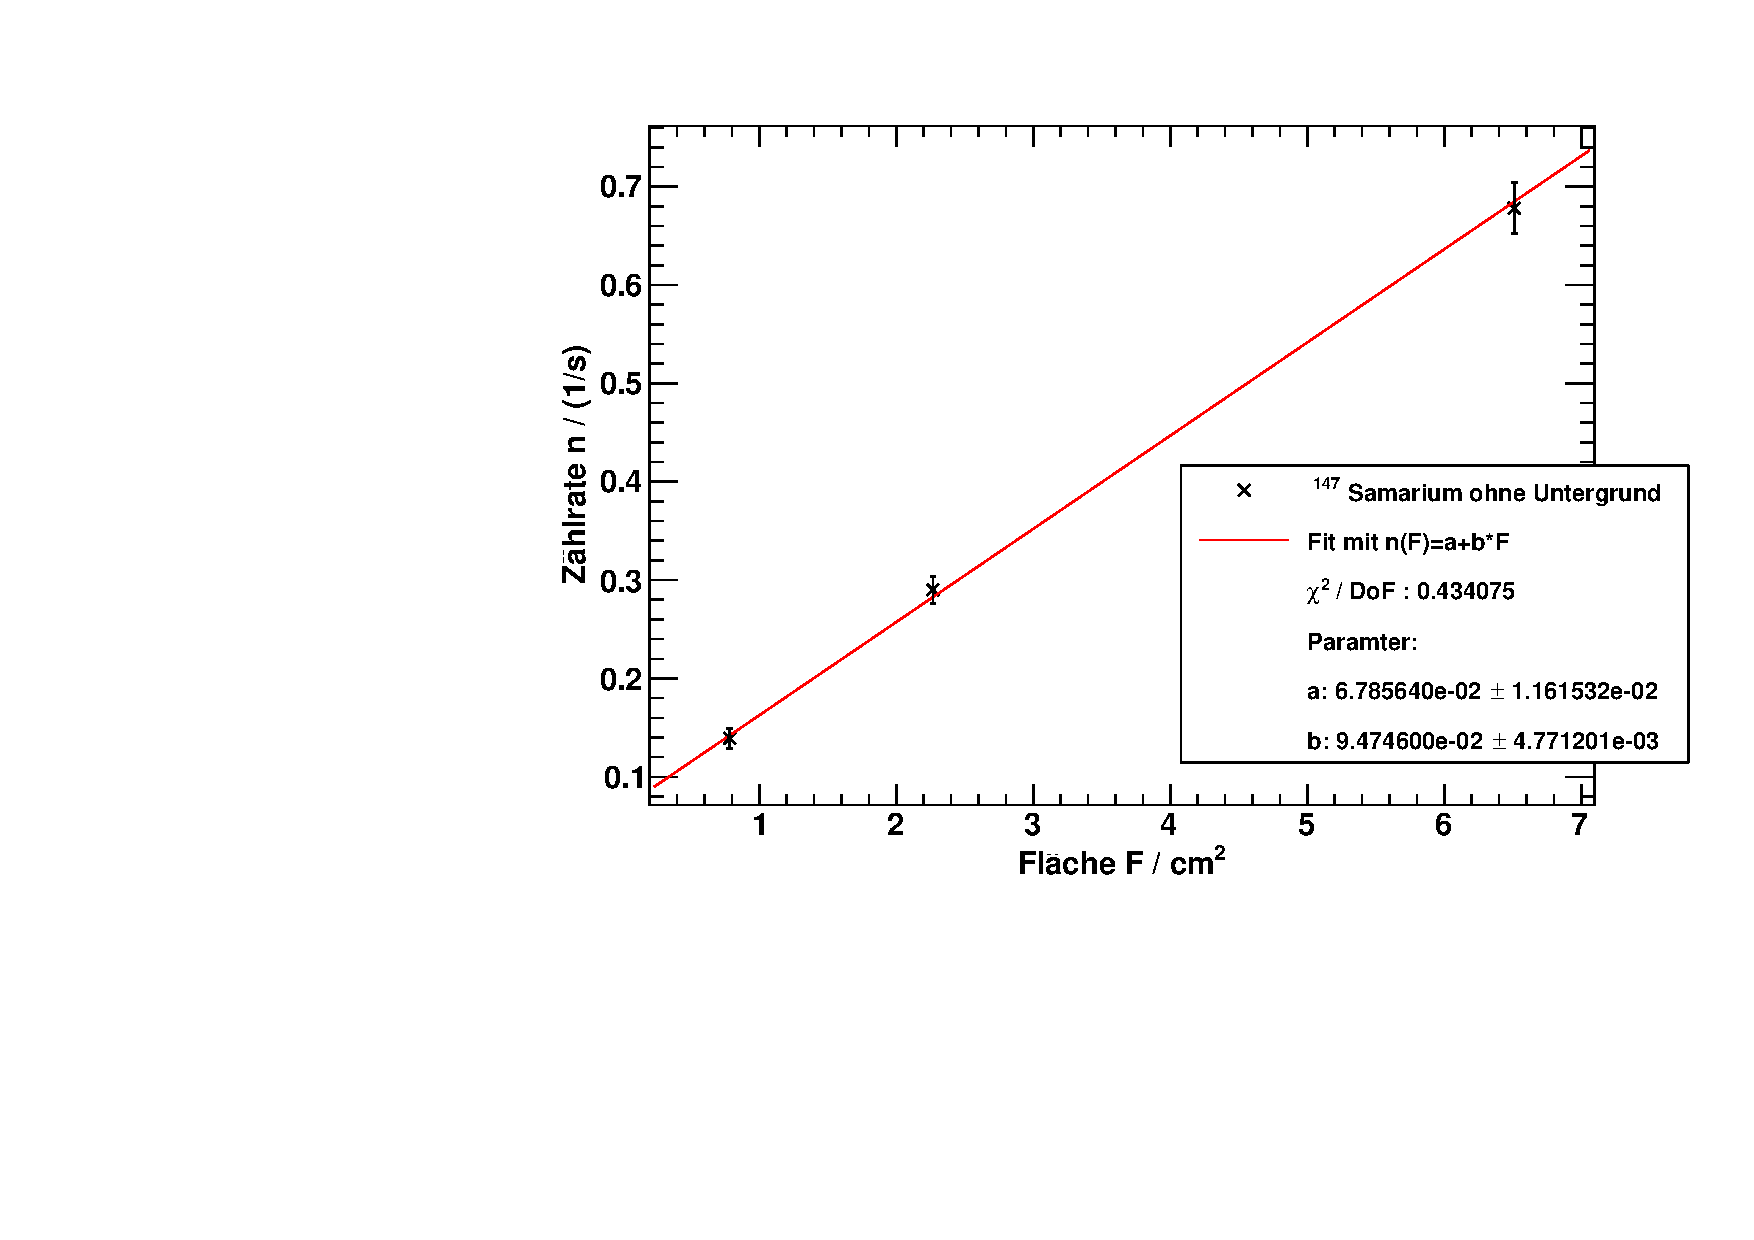
\includegraphics[width=15cm]{../img/Samarium147-Flaechenabhaengigkeit.pdf}
  \caption[Flächenabhängigkeit von \samarium]{Flächenabhängigkeit von \samarium\, bei 1600 V}
  \label{img:samarium:areafit}
\end{center}
\end{figure}
Die Rechnung liefert eine Halbwertszeit von
\begin{equation}
  T_{1/2}({}^{147}\text{Sm}) = (1.20 \pm 0.06) \cdot 10^{11} \text{ a}
\end{equation}

\subsubsection{Diskussion der Ergebnisse}
Der Literaturwert für die Halbwertszeit von \samarium\, ist $\tilde{T}_{1/2}({}^{147}\text{Sm}) = 1.06 \cdot 10^{11} \text{ a}$.
Wie schon in \ref{subsub:samarium:halflife:single} erwähnt, stimmen die Halbwertszeiten für die unterschiedlichen Flächen nicht miteinander 
überein. Der Wert für die größte Fläche $T_{1/2}(F=6.5106 \text{ cm}^2) = (1.09 \pm 0.04)\cdot 10^{11} \text{ a}$ stimmt innerhalb einer 
Standardabweichung mit dem Literaturwert überein, die Werte der anderen Flächen weichen jedoch stark von ihm ab. Wir vermuten einen systematischen 
Fehler (TODO Ursachen) \\%TODO Ursachen
Bei der Bestimmung der Halbwertszeit mit der Ausgleichsgeraden errechnet man einen Wert von 
$T_{1/2}({}^{147}\text{Sm}) = (1.20 \pm 0.06) \cdot 10^{11} \text{ a}$, welcher innerhalb von drei Standardabweichungen mit dem Literaturwert 
übereinstimmt. Der Achsenabschnitt sollte laut theoretischem Modell verschwinden, jedoch beträgt er $a = (0.068  \pm 0.012 ) \cdot \frac{1}{\text{s}}$
Dies könnte auf einen systematischen Fehler hinweisen.
%TODO Chi^2

\subsection{Bestimmung der Halbwertszeit von \kalium}
Auch in diesem Abschnitt sind alle Zählraten bereits die echten Zählraten und nach dem Verfahren, das in \ref{sub:eval:uran} beschrieben wurde, 
berechnet.
\subsubsection{$\beta$-Plateau von \kalium}
\begin{figure}[H]
\begin{center}
  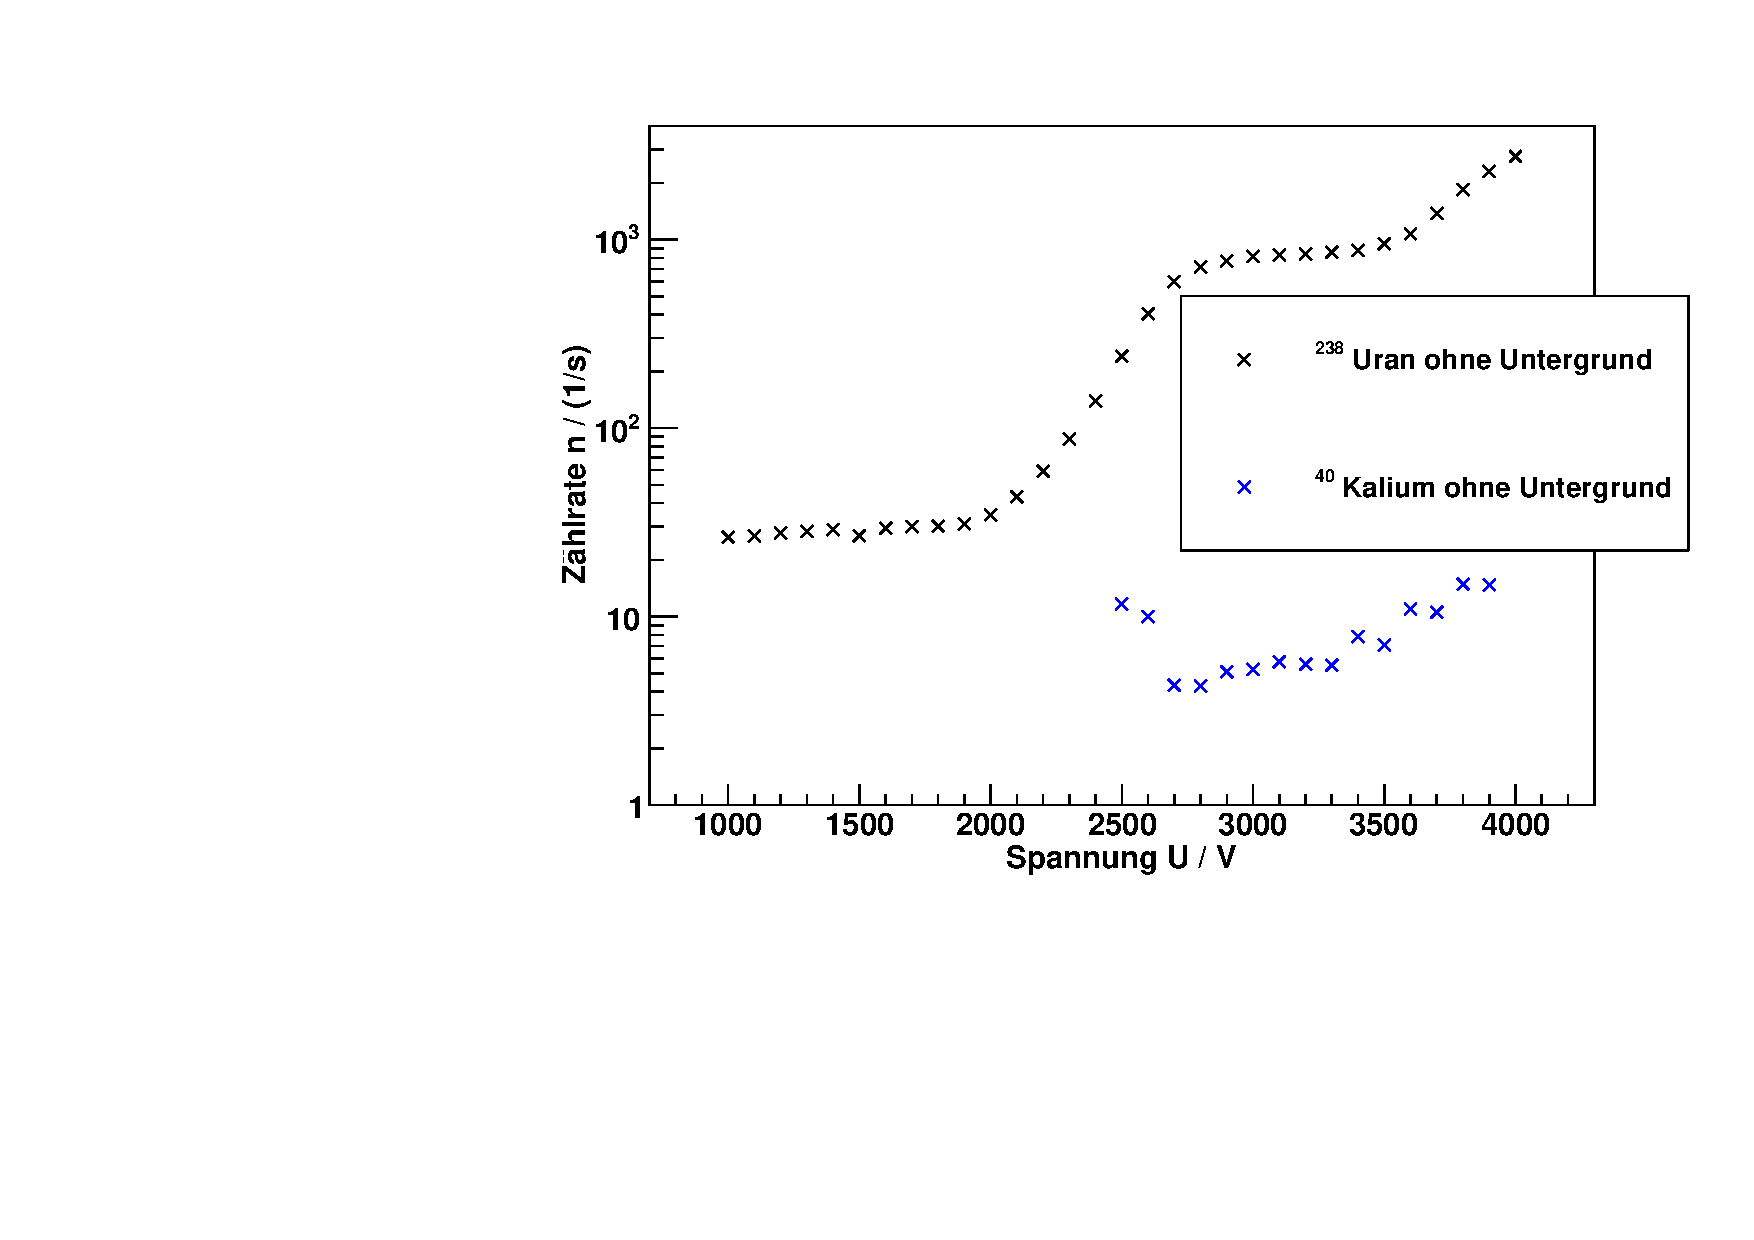
\includegraphics[width=15cm]{../img/Kalium40_Charakteristik.pdf}
  \caption[$\beta$-Plateau mit \kalium]{$\beta$-Plateau von \kalium}
  \label{img:char:kalium}
\end{center}
\end{figure}
In \autoref{img:char:kalium} ist das $\beta$-Plateau der Zählrate $n$ von \kalium\, ohne Untergrund gegen die Zählrohrspannung $V$ aufgetragen 
und in Vergleich mit der Zählrate von \uran\, gesetzt worden. Man erkennt das $\beta$-Plateau von $2700V$ bis ca. $3300V$. Danach steigt die 
Zählrate an, da die Spannung zu hoch für ein Proportionalzählrohr ist und man in den Bereich begrenzter Proportionalität gelangt. Die hohen Werte 
am Anfang sind durch kurzzeitige Schwankungen in der Zählrate zu erklären. Um eine Kurve mit weniger Schwankungen zu erhalten, müsste man bei den 
einzelnen Spannungen längere Messungen durchführen.

\subsubsection{Massenabhängigkeit der Zählrate} %TODO besserer Titel?
Nach \autoref{eq:kalium:countrate} hängt die Zählrate folgendermaßen von der Masse der Probe ab:
\begin{equation}
  n(m) = \frac{f}{2} \frac{A_s \cdot F \cdot \rho}{\mu} \left( 1 - e^{- \frac{\mu \cdot m}{F \cdot \rho}} \right) = a(1-e^{-b \cdot m})
\end{equation}
mit
\begin{equation}
  a = \frac{f}{2} \frac{A_s \cdot F \cdot \rho}{\mu} \qquad \text{und} \qquad b = \frac{\mu}{F \cdot \rho}
\end{equation}
Die beiden Parameter $a$ und $b$ lassen sich mit einer Kurvenanpassung (siehe \autoref{img:kalium:massdep}) bestimmen. \\
Die Werte dafür sind in \autoref{tab:data:kalium} aufgelistet.
\begin{table}[H]
\caption{Z"ahlraten von \kalium\,f"ur verschiedene Massen mit Fehlern}
\begin{center}
\begin{tabular}{|c|c|c|c|}
  \hline
  Masse $m /$g & $s_m /$g & Z"ahlrate $n / (1/\text{s})$ & $s_n / (1/\text{s})$ \\ \hline 
  2.012 & 0.001 & 5.426 & 0.173 \\ \hline
  2.012 & 0.001 & 5.088 & 0.171 \\ \hline
  1.905 & 0.001 & 5.192 & 0.171 \\ \hline
  1.681 & 0.001 & 5.297 & 0.172 \\ \hline
  1.483 & 0.001 & 4.773 & 0.168 \\ \hline
  1.295 & 0.001 & 4.961 & 0.165 \\ \hline
  1.099 & 0.001 & 4.525 & 0.162 \\ \hline
  0.809 & 0.001 & 4.344 & 0.157 \\ \hline
  0.695 & 0.001 & 3.803 & 0.154 \\ \hline
  0.501 & 0.001 & 3.251 & 0.146 \\ \hline
  0.303 & 0.001 & 2.280 & 0.138 \\ \hline
\end{tabular}
\end{center}
\label{tab:data:kalium}
\end{table}
 
\begin{figure}[H]
\begin{center}
  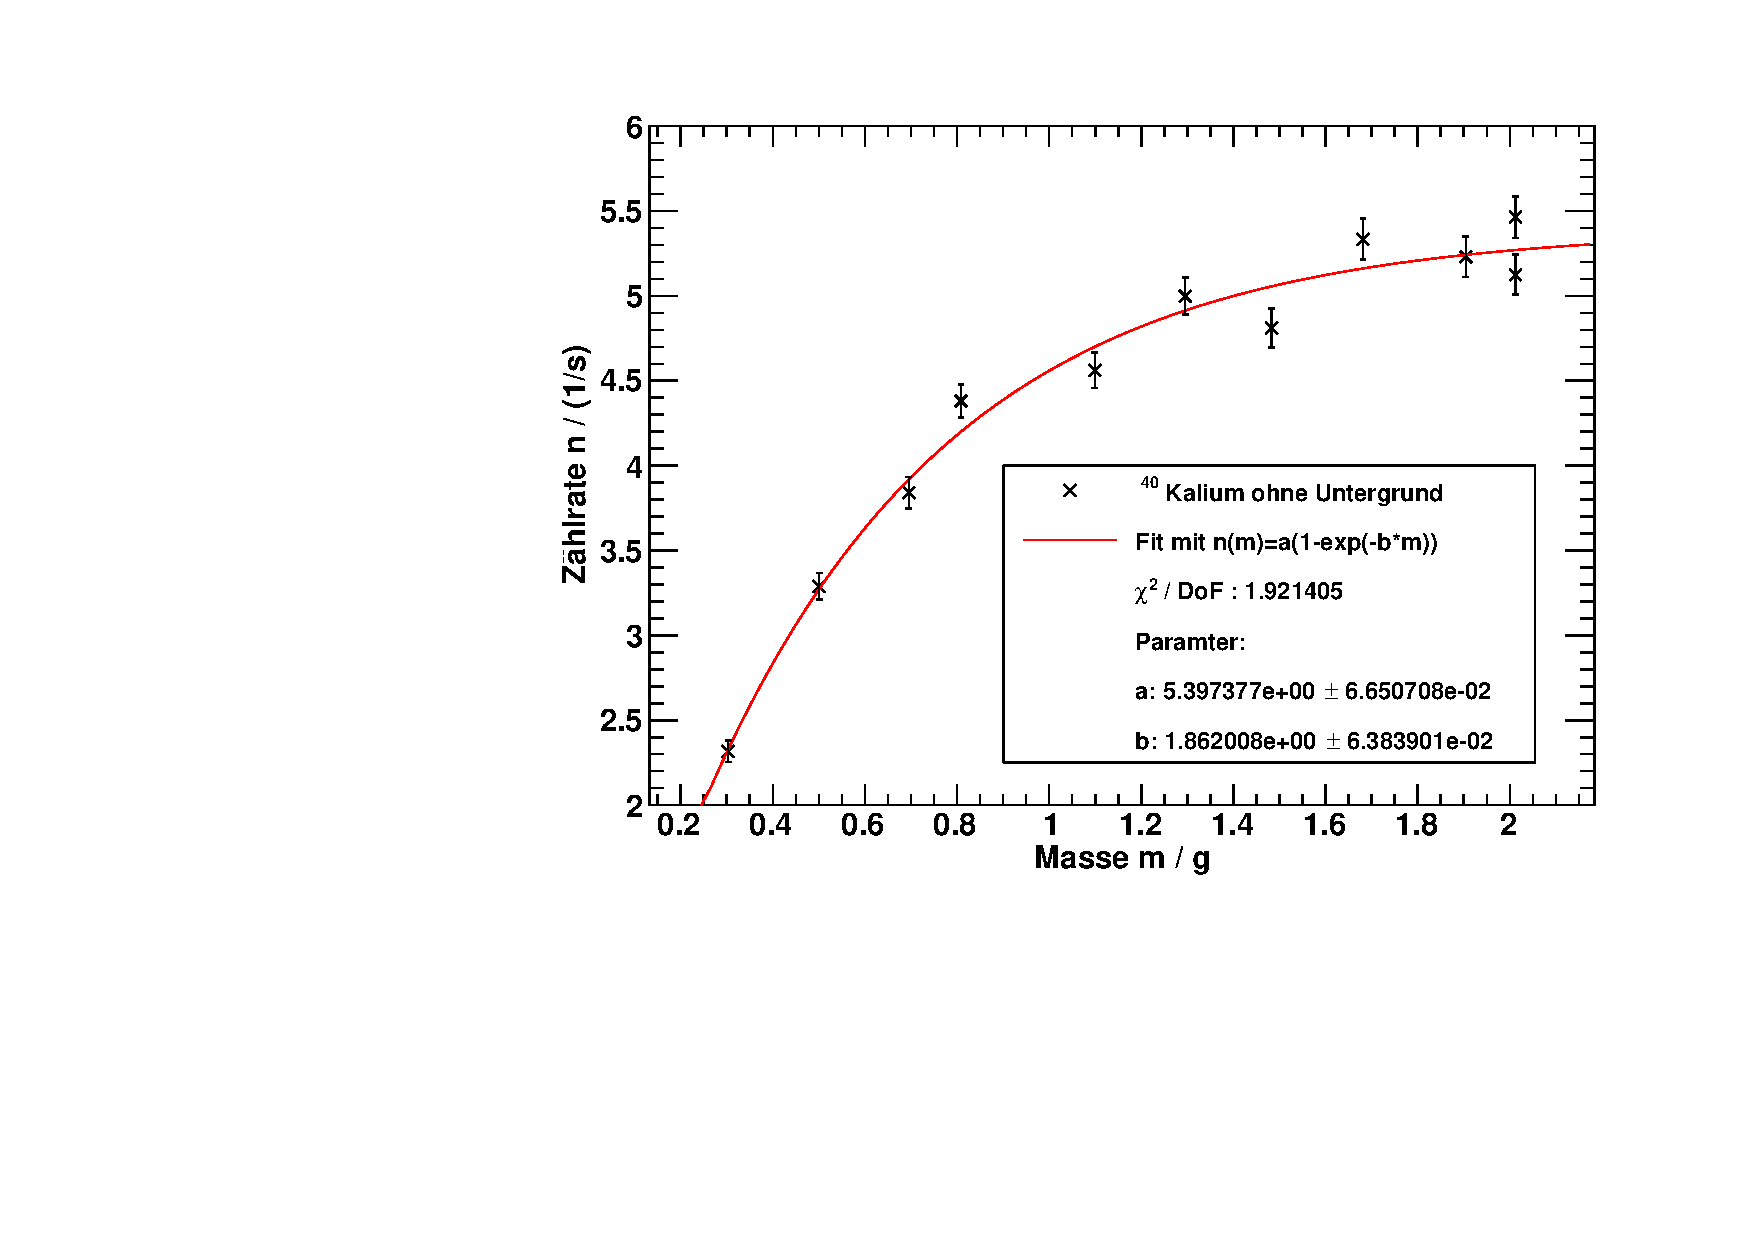
\includegraphics[width=15cm]{../img/Kalium40_Massenabhaengigkeit.pdf}
  \caption[Massenabhängigkeit der Zählrate von \kalium]{Massenabhängigkeit der Zählrate von \kalium\, bei 3200 V}
  \label{img:kalium:massdep}
\end{center}
\end{figure}
Die Werte lauten:
\begin{gather}
  a = (5.397 \pm 0.067) \cdot \frac{1}{\text{s}} \\ %TODO runden ja oder nein?
  b = (1.862 \pm 0.064) \cdot \frac{1}{\text{g}} 
\end{gather}
Außerdem ergibt sich ein Korrelationskoeffizient von
\begin{equation}
  \rho = \frac{\cov(a, b)}{\sigma_a \sigma_b} = -0.82
\end{equation}
%TODO Chi^2 / DoF Auswertung

\subsubsection{Berechnung der Halbwertszeit}
Aus dem Produkt der beiden Parameter lässt sich die spezifische Aktivität $A_s = \frac{A}{m}$ bestimmen:
\begin{equation}
  A_s = \frac{2 \cdot a \cdot b}{f} \quad \Rightarrow \quad A = m \cdot \frac{2 \cdot a \cdot b}{f}
\end{equation}
Es wird bei der Messung nur die $\beta^-$-Strahlung gemessen, allerdings tritt bei dem Zerfall von \kalium\, auch noch Elektroneneinfang auf. 
Das Verhältnis zwischen $\beta^-$-Zerfall und Elektroneneinfang beträgt $12\%$. Daher gilt für die Zerfallskonstante
\begin{equation}
  \lambda = \lambda_{\beta^-} + \lambda_{\text{EC}} = 1.12 \lambda_{\beta^-}
\end{equation}
Daher berechnet sich die Halbwertszeit von \kalium\, mit \autoref{eq:lambdahwz}
\begin{equation}
  T_{1/2}({}^{40}K) = \frac{\ln 2}{\lambda} = \frac{\ln 2}{1.12} \frac{1}{\lambda_{\beta^-}} = \frac{\ln 2}{1.12} \frac{N}{A}
\end{equation}
bestimmen. \\
Die Anzahl $N$ der Kaliumkerne in Kaliumchlorid ist:
\begin{equation}
  N = \frac{m \cdot N_A}{M_{KCl}} h_{\text{rel}}
\end{equation}
wobei $N_A$ die Avogadrokonstante, $M_{KCl}=74.5483\,u$ die molare Masse von Kaliumchlorid und $h_{\text{rel}}=0.0118\%$ die relative Anzahl von Kaliumkernen 
in Kaliumchlorid ist. \\
Daraus berechnet sich die Halbwertszeit von Kalium mit:
\begin{equation}
  T_{1/2} \left( {}^{40} K \right)  = \frac{\ln 2}{1.12} \frac{N_A \cdot h_{\text{rel}}}{M_{KCl}} \frac{f}{2} \frac{1}{a \cdot b} = const. \cdot \frac{1}{a \cdot b}
\end{equation}
Der Fehler ergibt sich aus den relativen Fehlern von $a$ und $b$ und der Berücksichtigung des Korrelationskoeffizienten $\rho$:
\begin{equation}
  \sigma_{T_{1/2}} = \sqrt{ \left( \frac{\sigma_a}{a} \right)^2 + \left( \frac{\sigma_b}{b} \right)^2 + 2 \cdot \frac{\sigma_a}{a} \cdot \frac{\sigma_b}{b} \cdot \rho   }
\end{equation}
Man erhält folgendes Ergebnis:
\begin{equation}
  T_{1/2} \left( {}^{40} K \right) = (1.20 \pm 0.03) \cdot 10^9\,\text{a}  
\end{equation}

\subsubsection{Diskussion des Ergebnisses}
